The current implementation, while functional, is far from optimal. There are bottlenecks which restrict performance and the system is unstable. It is not feasible to build a system as fast and as performant and stable as \ceph{} or \ac{hdfs} within the scope of a thesis to. Here I have explored whether an architecture using ministries and ranged based file locking offers an advantage to existing solutions. We can still answer that question given these restrictions.

Before we can design experiments that work around the limitations we need to be clear on what the limitations are:

\begin{itemize}
	\item The \raft{} implementation sends only a single log entry at the time and log entries are sent each heartbeat period instead of whenever data becomes available. Effectively this imposes a rate limit on the number of changes made to metadata.
	\item Load balancing only replaces nodes that go down, it does not perform subtree partitioning at runtime (see:~\Cref{sec:subtree}).
	\item Sometimes nodes become unresponsive when making many requests that change metadata. They then miss heartbeats which triggers re-elections.
\end{itemize}

Firs we look at the \textit{ministry architecture} tracking how performance changes when we change the number of ministries. Then we look at \textit{ranged based file locking} by comparing write performance with and without locking. Every benchmark was performed five times and all the results are presented. All nodes where monitored during each run and if an error occurred we repeated the entire run. The raw data is available \href{https://github.com/dvdsk/Thesis}{github.com/dvdsk/Thesis}.

All the benchmarks have been performed using the fifth generation distributed ASCI Supercomputer \cite{das5}. Each node has a Dual eight-core Intel Xeon E5-2630 v3 and 125G of ram. The system is equipped with InfiniBand however we use the normal Ethernet networking as networking delays are a key characteristic of the systems' performance.

\subsection{Ministry Architecture}
Here we test the impact of varying the number of ministries on performance. We expect to see an almost linear improvement with more ministries given optimal size and shape of the load.

Live subtree partitioning is still unimplemented we work around this by implementing static subtree partitioning. The load balancer starts by initializing a single ministry responsible for the root directory. Additional static ministries can be passed through command line parameters. For these test we let it initialize n-1 ministries at paths \textsl{/n}.

\subsubsection{List directory}
To test performance we perform 60 thousand ls requests for various directories from 30 clients concurrently. Each client sends the requests one after another as fast as possible. To keep the overhead from sending back the directory content each directory contains only 10 files. The client processes are spread between 3 physical nodes.

The 2000 ls requests each client sends are in two different orders: \textit{batch} and \textit{stride}. In \textit{batch} a client performs all the ls requests for a single directory before sending those for the next. When using the \textit{stride} pattern a client sends a request to the first directory and then sends the next request to another directory. The results below hide extreme outliers two standard deviations outside the mean which are requests taking longer then 2ms.

In \Cref{fig:ls_vs_ministries} we see a violin plot comparing the two request orders for clusters with various number of ministries. On the Y-axis we see the time it took a single request to complete. A wider distribution means more requests where completed within the same time. Note the multimodal distribution, the increasing duration for the slowest requests as the number of ministries increases and the difference in the fastest times between batch and stride. Outliers further out then $4\sigma$ are not shown.

\Cref{fig:ls_cdf} shows \acp{cdf} of clients performing 60 thousand list directory requests in \textit{batch} mode for varying amount of ministries. On the Y-axis are the proportion of requests that complete within the time on the X-axis. Note using 1 ministry is always the fastest followed initially by 5 ministries until 80% of te requests complete at which point it becomes the slowest.

\begin{figure}[bp]
	\centering
	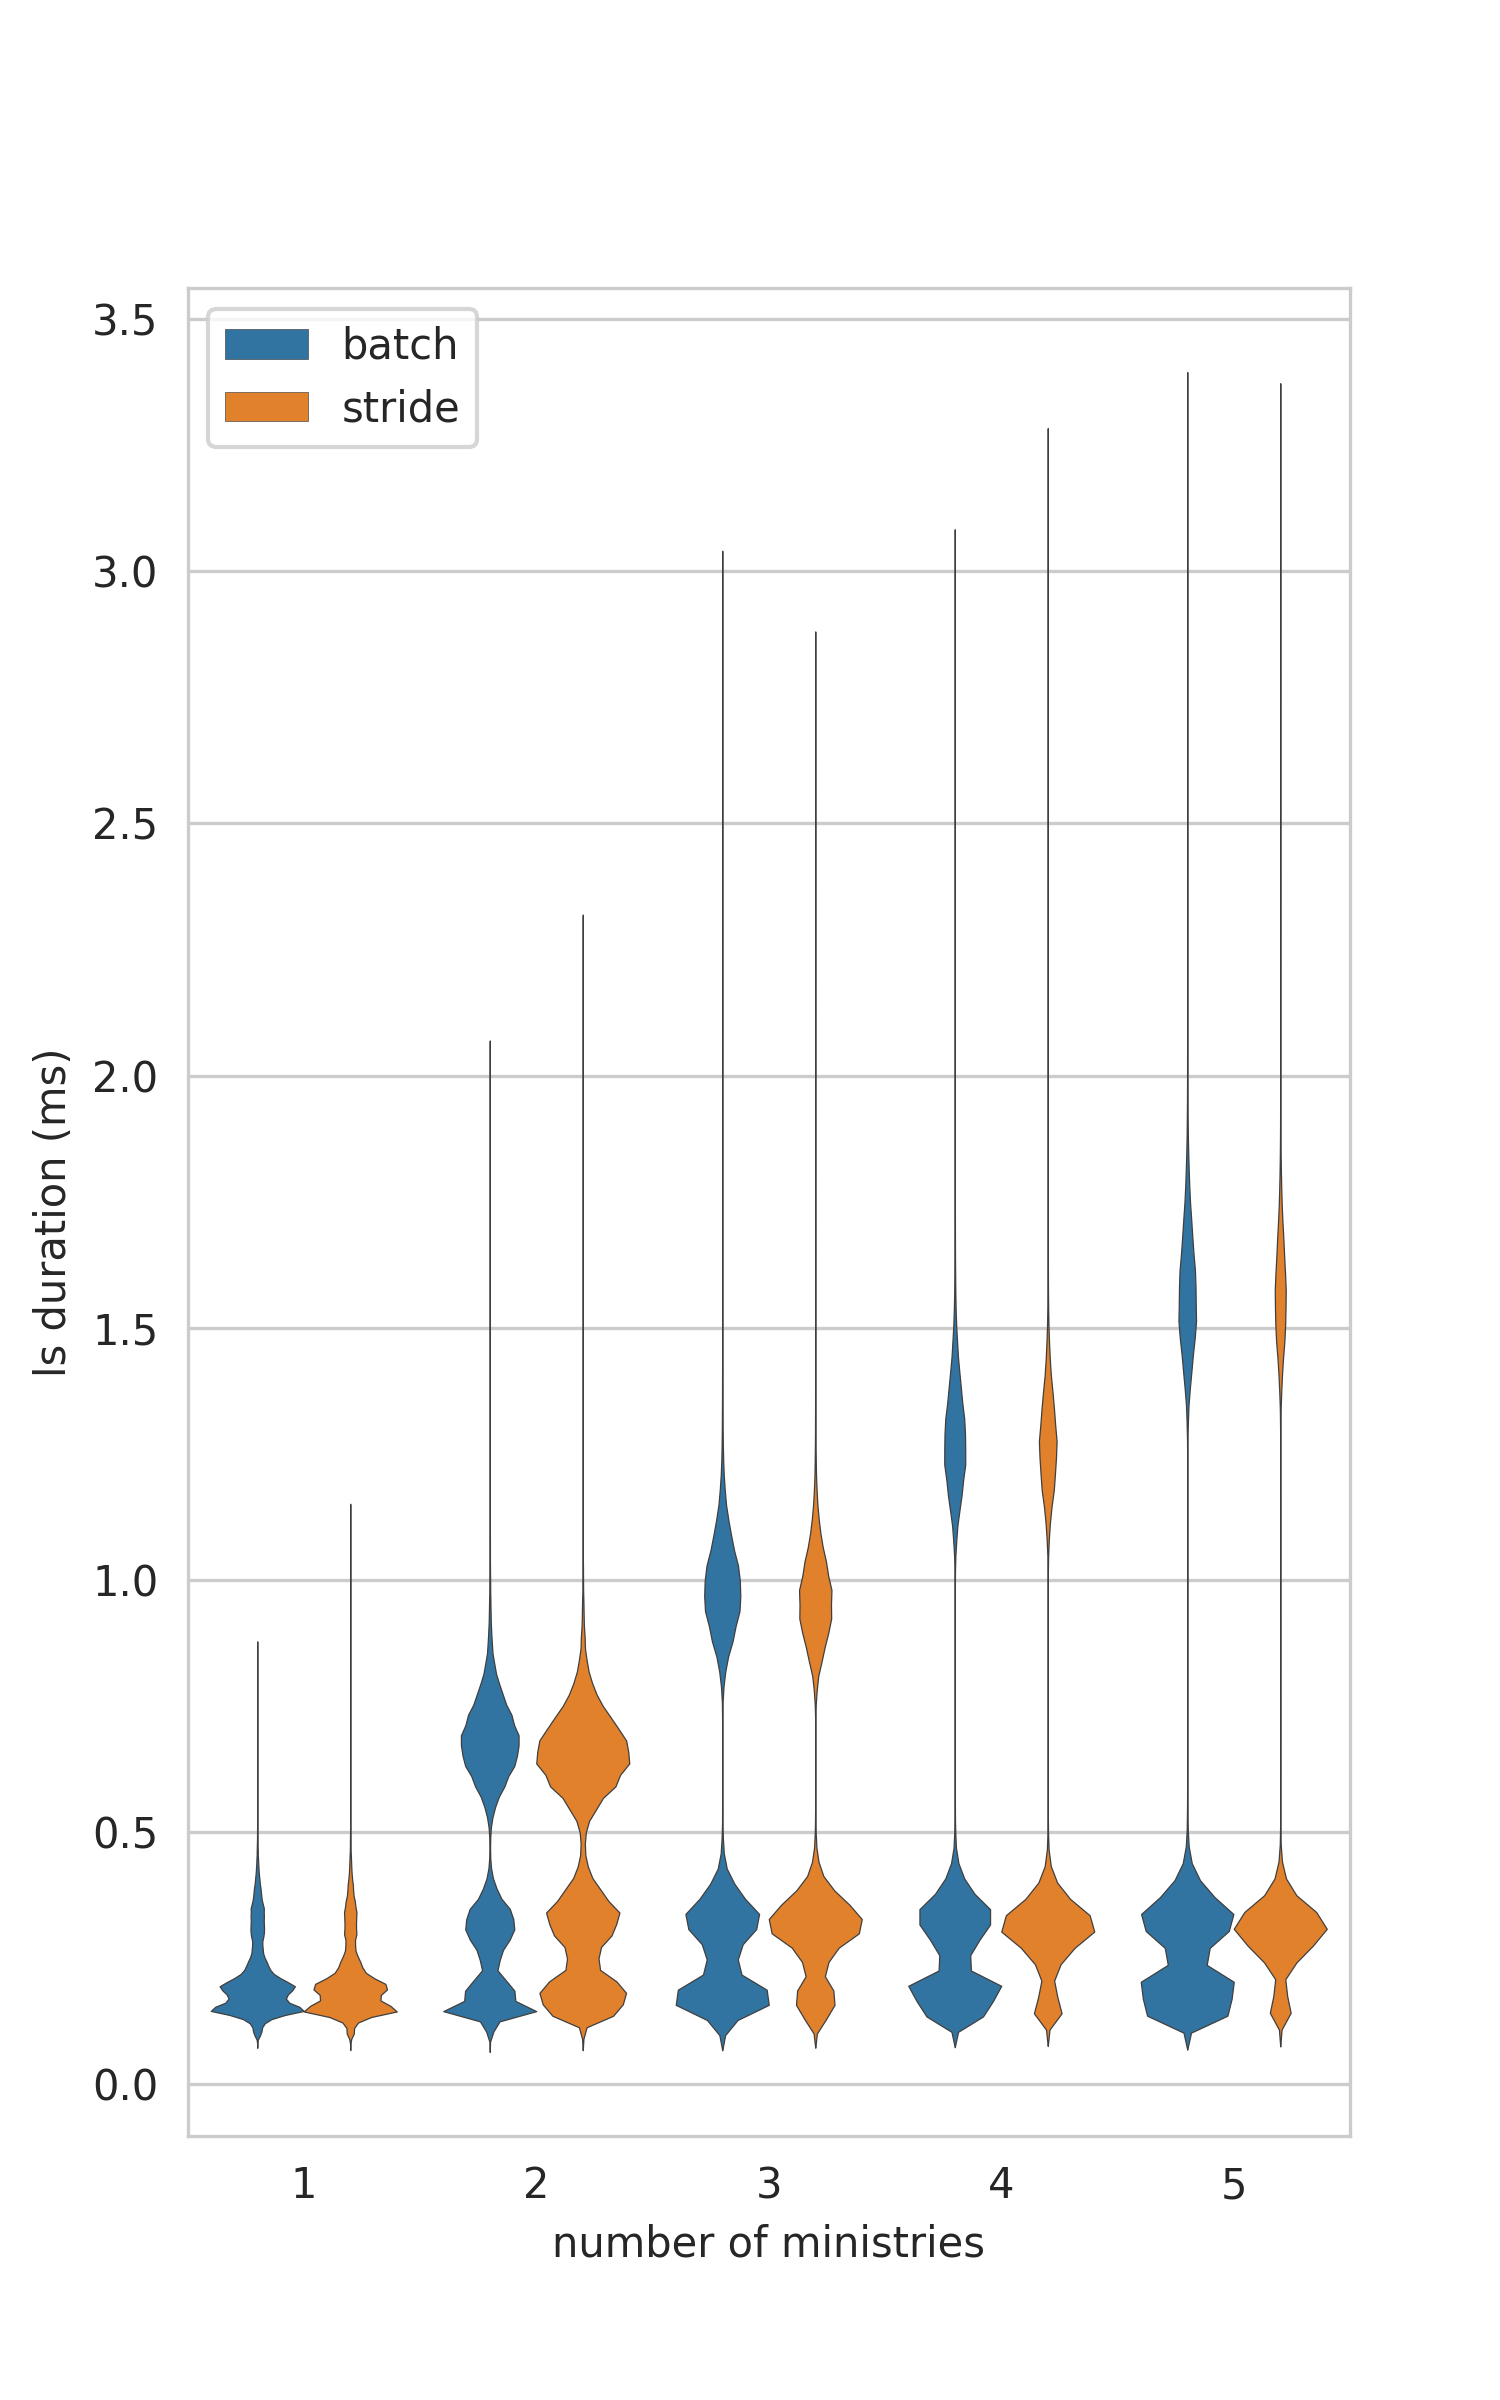
\includegraphics[height=\textheight]{../results/plots/ls_vs_numb_ministries.png}
	\caption{Distribution of list directory duration vs number of ministries for two different request orders. On the Y-axis the time it takes a single request to complete. The X-axis shows the number of ministries the file system is using. The orange distributions are results from runs where $30$ clients ordered their request such that the ministries where accessed one after the other, a stride pattern. The Blue distributions show results from runs where $30$ clients used a batch pattern: they first perform all requests for one ministry and then for the next. Outliers further out then $4\sigma$ are not shown}
	\label{fig:ls_vs_ministries}
\end{figure}%

\begin{figure}[htb]
	\centering
	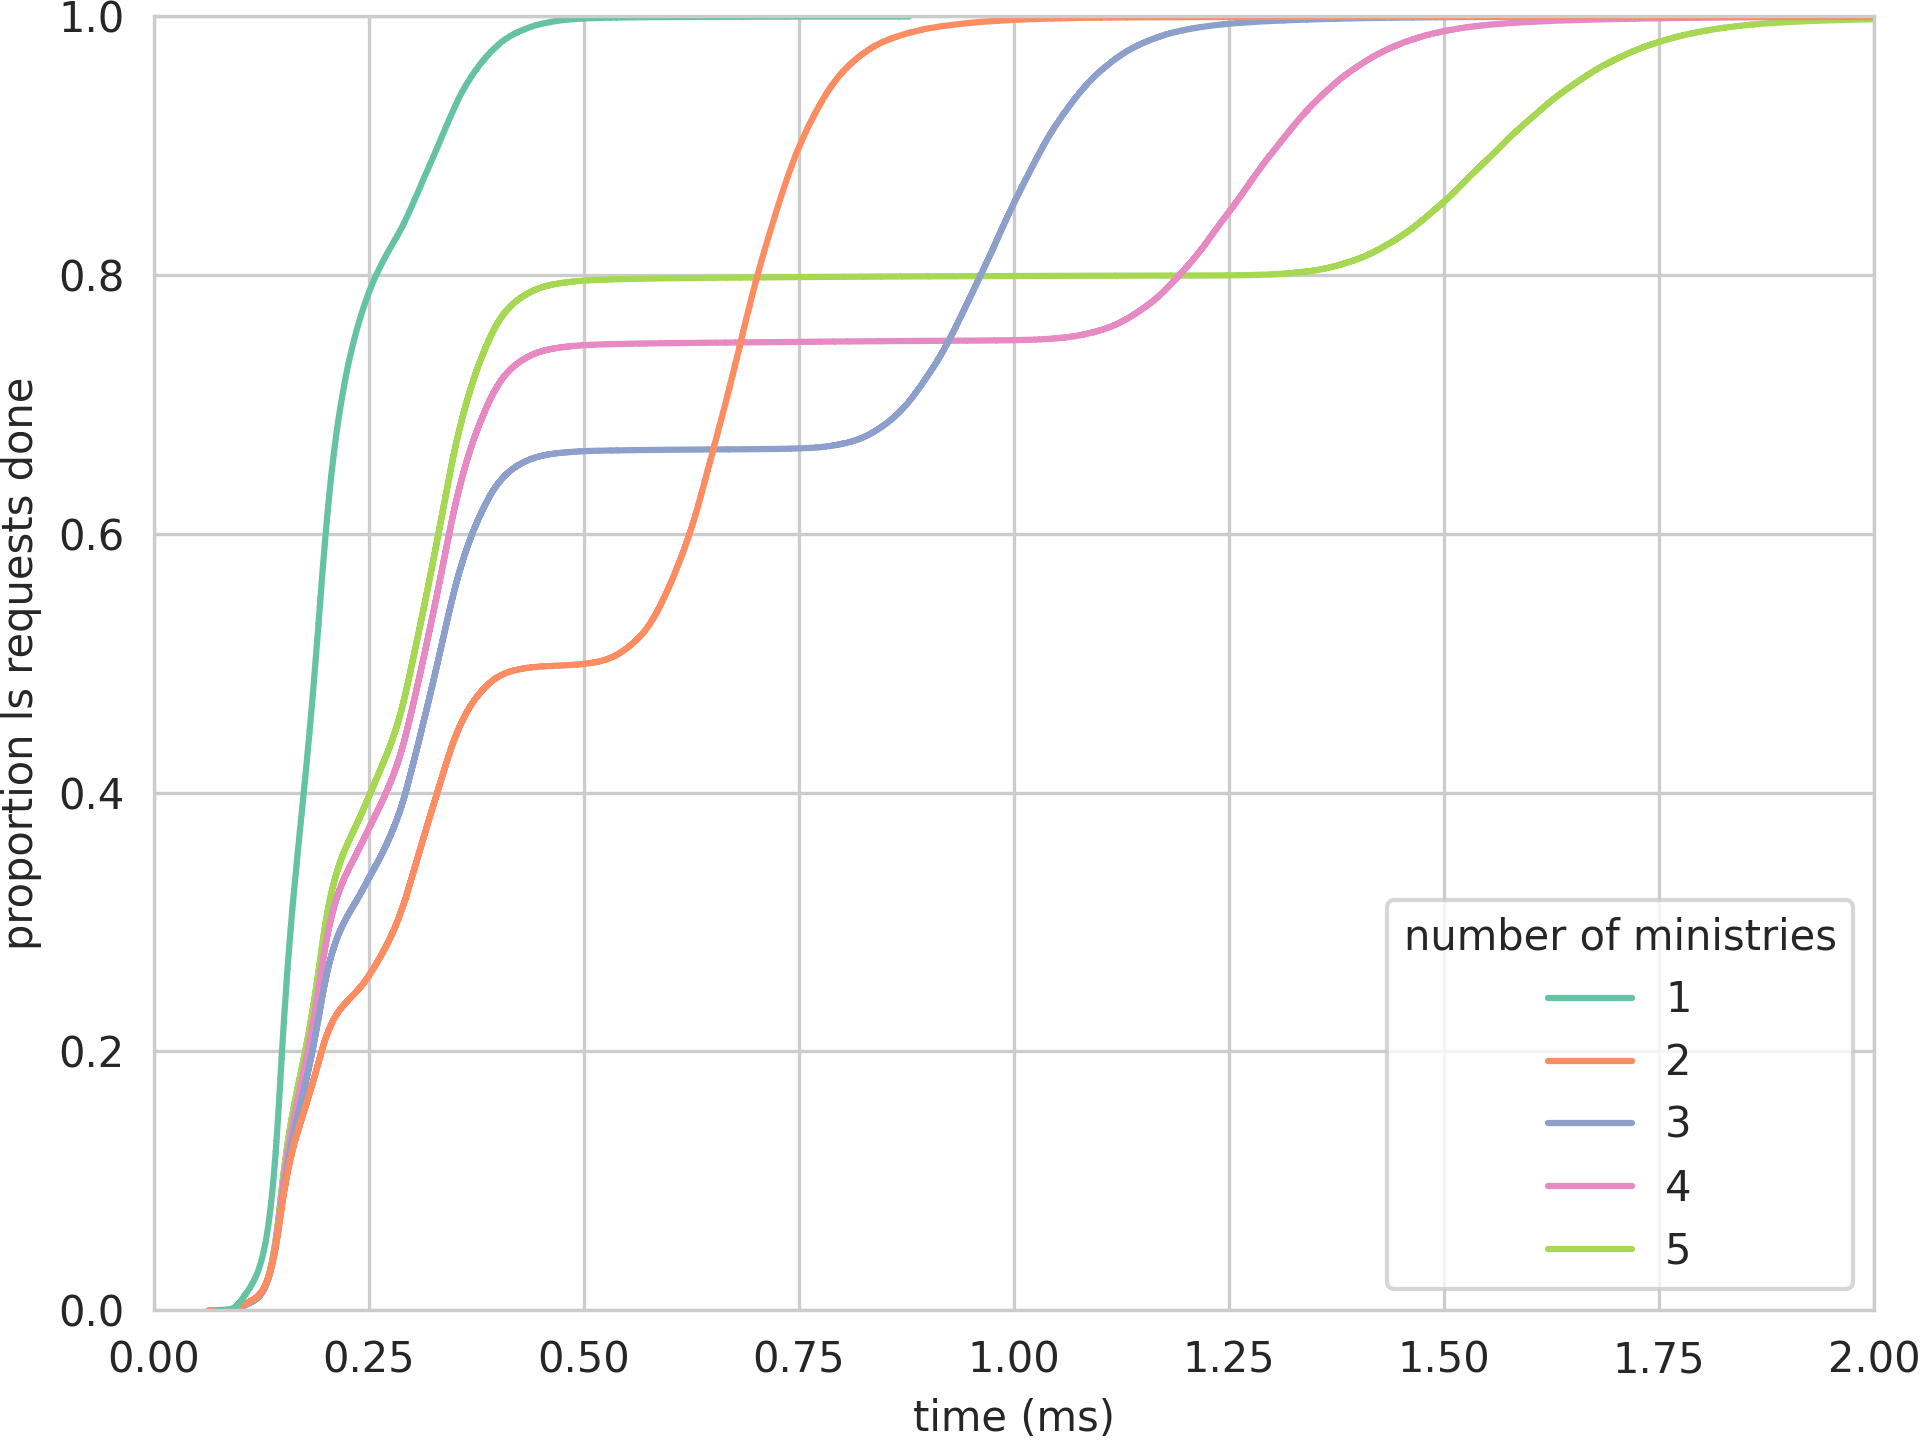
\includegraphics[height=\textheight]{../results/plots/ls_batch.png}
	\caption{\acp{cdf} of clients performing 60 thousand list directory requests for varying amount of ministries. On the Y-axis the proportion of requests completed, at $1.0$ all 60 thousand requests have been answered. The X-axis shows the time until the proportion was reached. The clients batch ordered their requests: they first perform all requests for one ministry and then for the next.}
	\label{fig:ls_cdf}
\end{figure}

\clearpage{}
\subsubsection{Create file}
The current implementation effectively imposes a rate limit on the log. To create a file a minister appends a single message to the log, this makes creating files also rate limited. Without this rate limit load could increase until the communication with the clerks or the hardware of the nodes becomes the bottleneck.%
%\footnote{That is assuming there are no other bottlenecks. We investigate this by profiling the nodes, see:~\Cref{sec:profile}} % % TODO: re-enable if we have time/it is possible to present the profiling results <04-08-22> 

It is interesting therefore to see how the performance scales with the number of ministries as more ministries would  solve future bottlenecks.

Because of the rate limit we send only 90 create requests. They are sent from 9 clients concurrently. These numbers where empirically determined to maximize the load while keeping the cluster stable enough to complete all the tests.

In \Cref{fig:touch} we see \acp{cdf} for creating files with various number of ministries. On the Y-axis the proportion of write requests completed and on the X-axis the time in milliseconds. Note the minimal latency creating a request is about 70 milliseconds. Furthermore, the more ministries we use the faster most requests are done. Finally, note the proportion of requests to complete jumps up in discrete for each configuration.

\Cref{fig:touch_vs_time} offers another look at the same data. Here we see the time needed for each request as a function of when the request started. Darker tones are requests from tests with more ministries. On the Y-axis we see the time needed to complete the request in seconds while on the (logarithmic) X-axis we see the time a request was sent. The vertical jumps in the \ac{cdf} (\Cref{fig:touch}) show up as horizontal bands here. For example the lowest horizontal band are requests that took 70 ms which matches the first vertical jump. Note that the gap just after the start of the test. It is consistent with requests taking at least 70ms.

\begin{figure}[htbp]
	\centering
	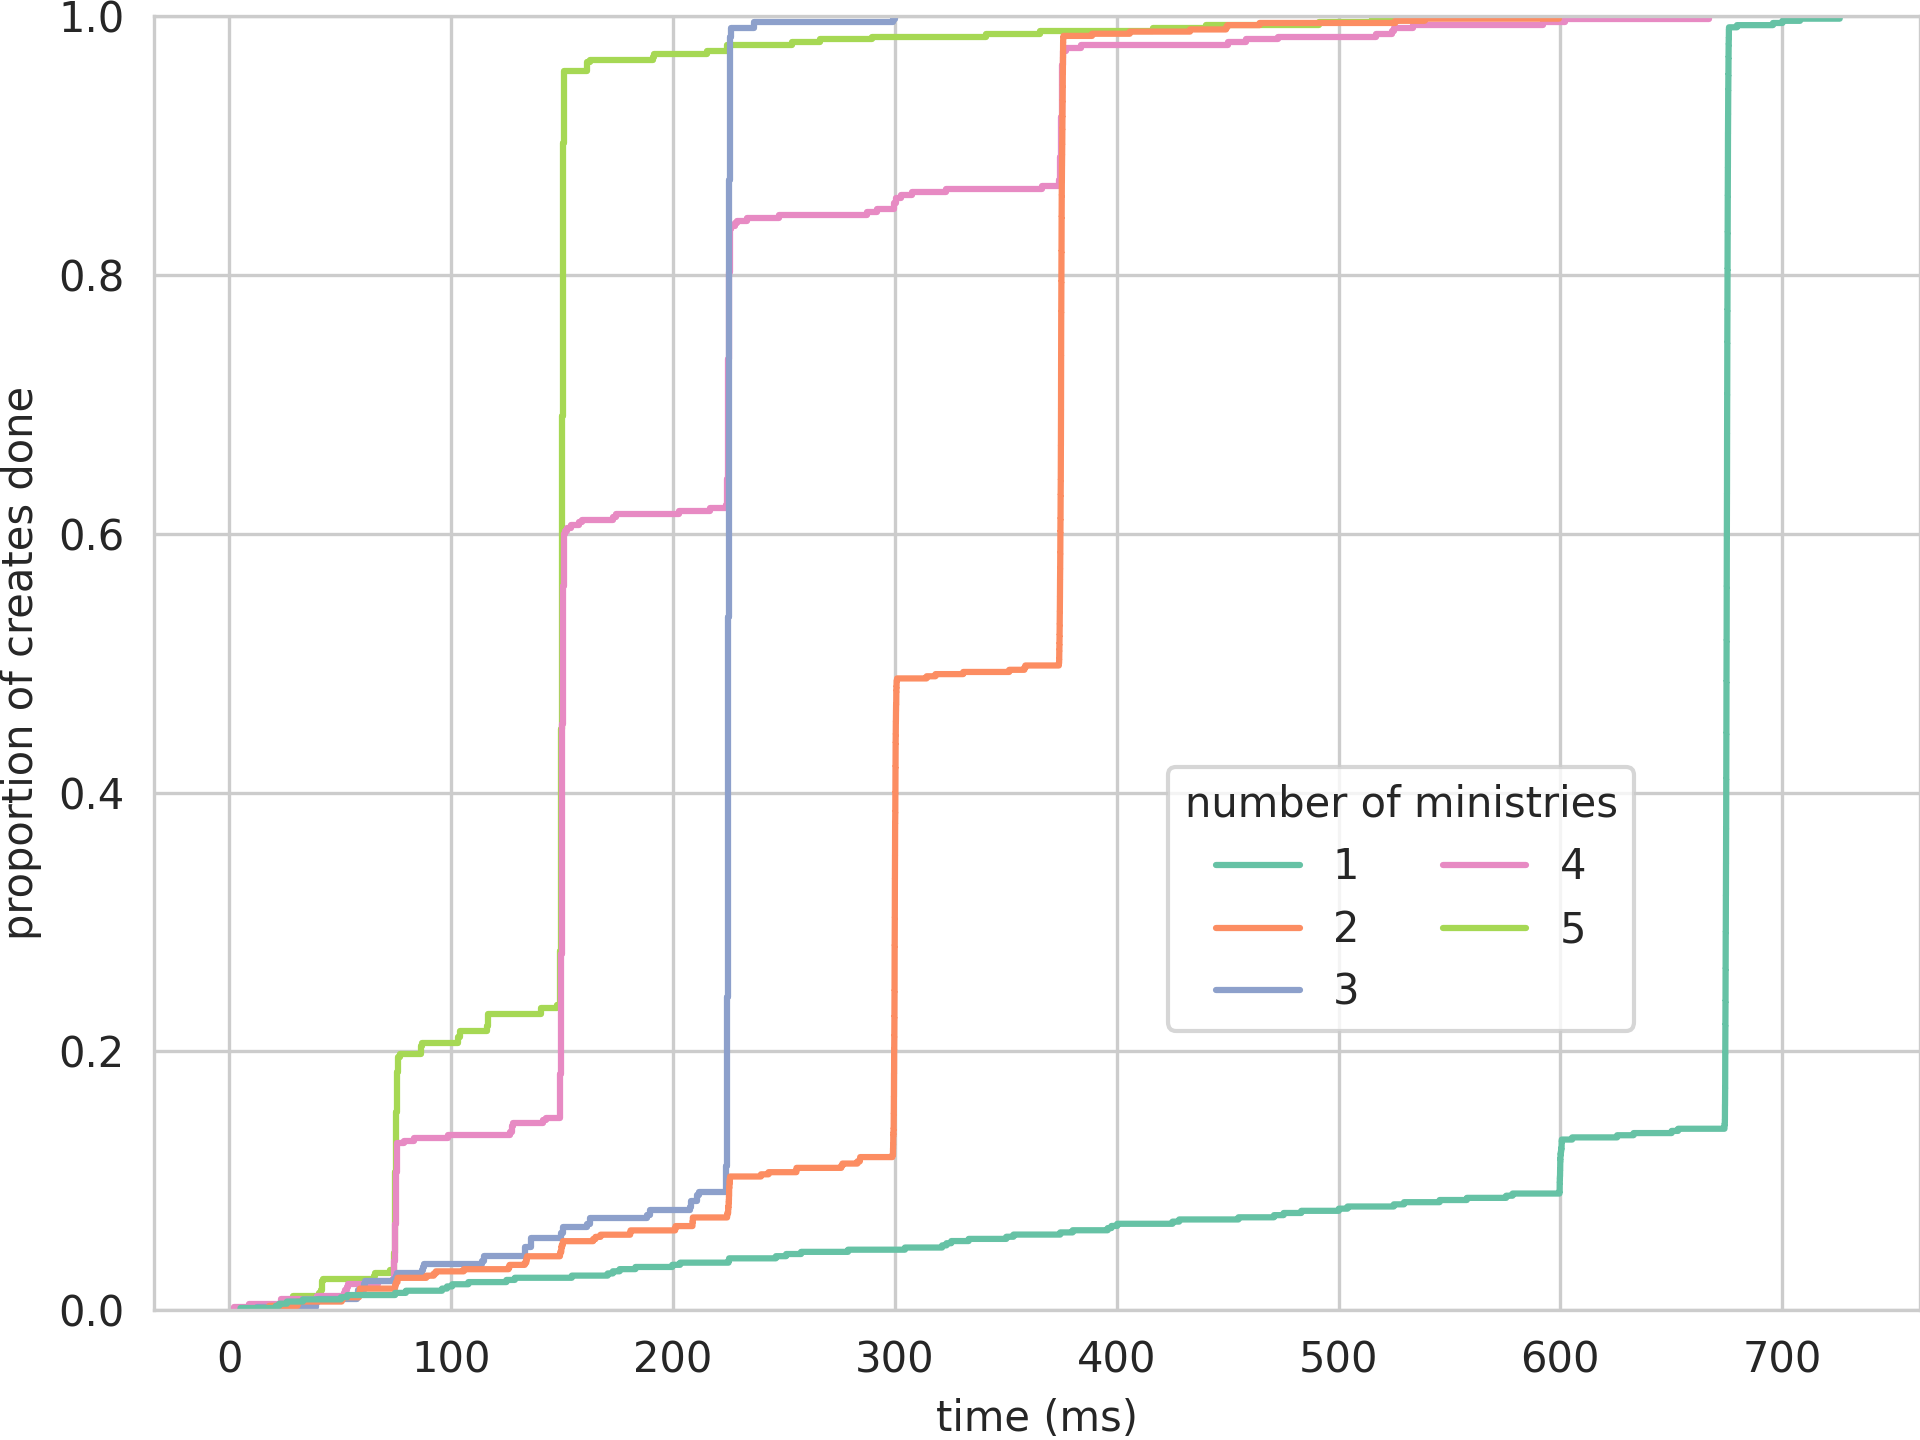
\includegraphics[height=\textheight]{../results/plots/touch.png}
	\caption{\acp{cdf} of clients creating 90 files on clusters with various amount of ministries. On the Y-axis the proportion of files created, at $1.0$ all 90 files have been created. On the X-axis the time in milliseconds until that proportion was reached.}
	\label{fig:touch}
\end{figure}

\begin{figure}[bp]
	\centering
	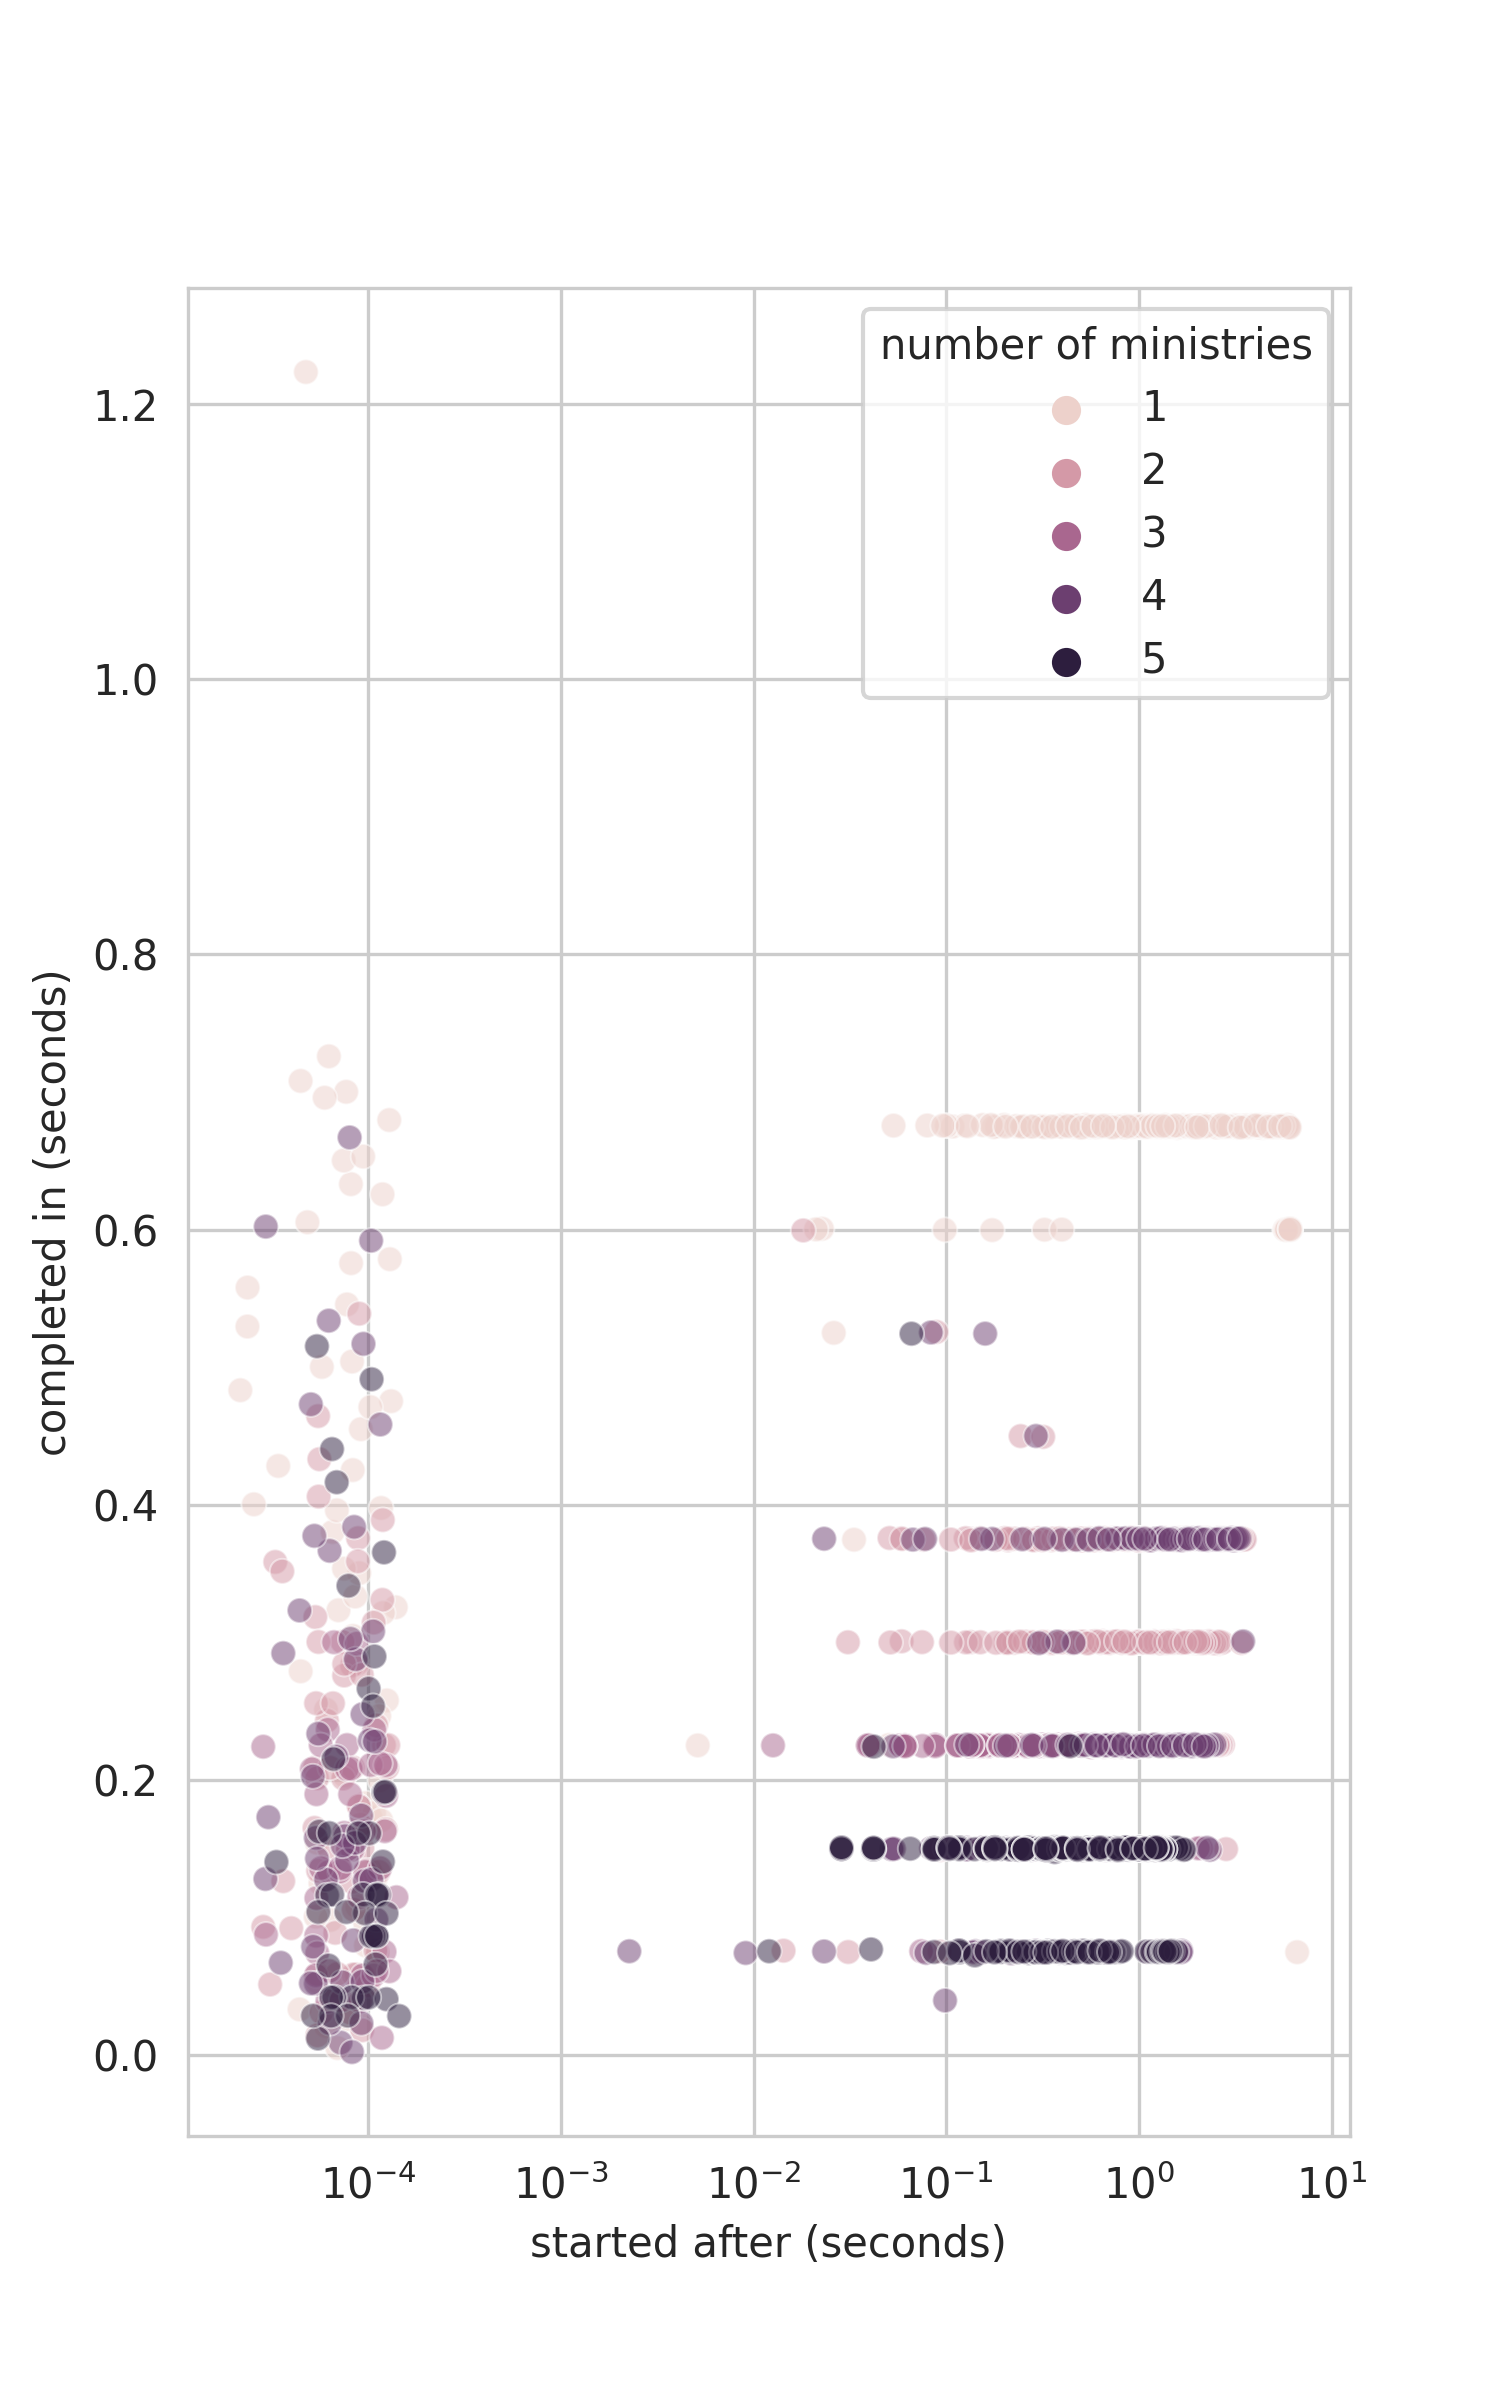
\includegraphics[height=\textheight]{../results/plots/touch_vs_time.png}
	\caption{A logarithmic plot of file create request time vs when the request was started. The same data as in \Cref{fig:touch}. On the Y-axis the time it took a request to complete in seconds while the X-axis shows the point at which the request was started. Darker points are requests made to clusters with more ministries.}
	\label{fig:touch_vs_time}
\end{figure}

\clearpage{}
\subsection{Range based file locking}
We evaluate the contribution of ranged writes vs writing to the entire file. A good use case of ranged file access is writing out one or more rows in a file that consists of equally sized rows. We can do this by requesting exclusive access to the entire file and writing out all the needed rows. Alternatively we can request access to and writing out one row at the time. We expect the second method to be faster when contending with more clients for the same file and with larger files.

Here we benchmark these different methods using two different. First we look at writing a single row of a file with 10 rows in total from multiple clients simultaneously. Secondly we try writing all rows again from multiple clients simultaneously. When accessing and writing by row each client uses a random order. For the experiments where we write only a single row this means the row is chosen at random.

We see how performance changes when changing the row size or number of concurrent writers. For the results over varying row size 6 concurrent writers where used. When changing the number of writers the row size was kept at 10 \ac{mby}.

Since \name{} has no data plane writing is simulated by sleeping on the client side. We simulate writing at a speed of 200 \ac{mby} per second\footnote{This corresponds to a slow hard drive. That is the best case scenario for writing by row since it increases the ration of time writing versus connecting and locking the file}.

In the table below we see the time spend on simulating IO and the average duration for writing one or 10 rows either by locking the whole file or locking by row.
%
\begin{tabular}{lcccccc} \toprule
	& \multicolumn{6}{c}{Row Size (\ac{mby})} \\ \cmidrule(r){2-7}
	                   & 0.1 & 1 & 10 & 20 & 40 & 80 \\ \midrule
	Writing a single row  \\ \cmidrule(r){1-1}
	IO simulation (ms) & 0.5          & 5          & 50          & 100         & 200         & 400 \\
	Lock by row & 411 & 370 & 366 & 444 & 636 & 971\\
	Lock entire file & 62 & 114 & 298 & 618 & 975 & 1644 \\
\smallskip \\
	Writing 10 rows (s)\\ \cmidrule(r){1-1}
	IO simulation & 0.005          & 0.05          & 0.50          & 1         & 2         & 4 \\
	Lock by row & 2.83         & 3.00       & 3.52        & 4.58        & 7.29        & 12.12 \\
	Lock entire file & 0.57         & 0.82       & 1.51        & 2.65        & 4.90        & 9.60 \\ \bottomrule
\end{tabular}
%
\subsubsection{Writing a single row}
%
\Cref{fig:single_rowlen} shows the time it takes to write a single row for different row sizes. The Y-axis shows the duration a single write request takes in seconds. Each dot is a single measurement. We see that locking the entire file is slower than locking only the needed row. Note how increasing the row length shrinks the performance gap.

\begin{figure}[htbp]
	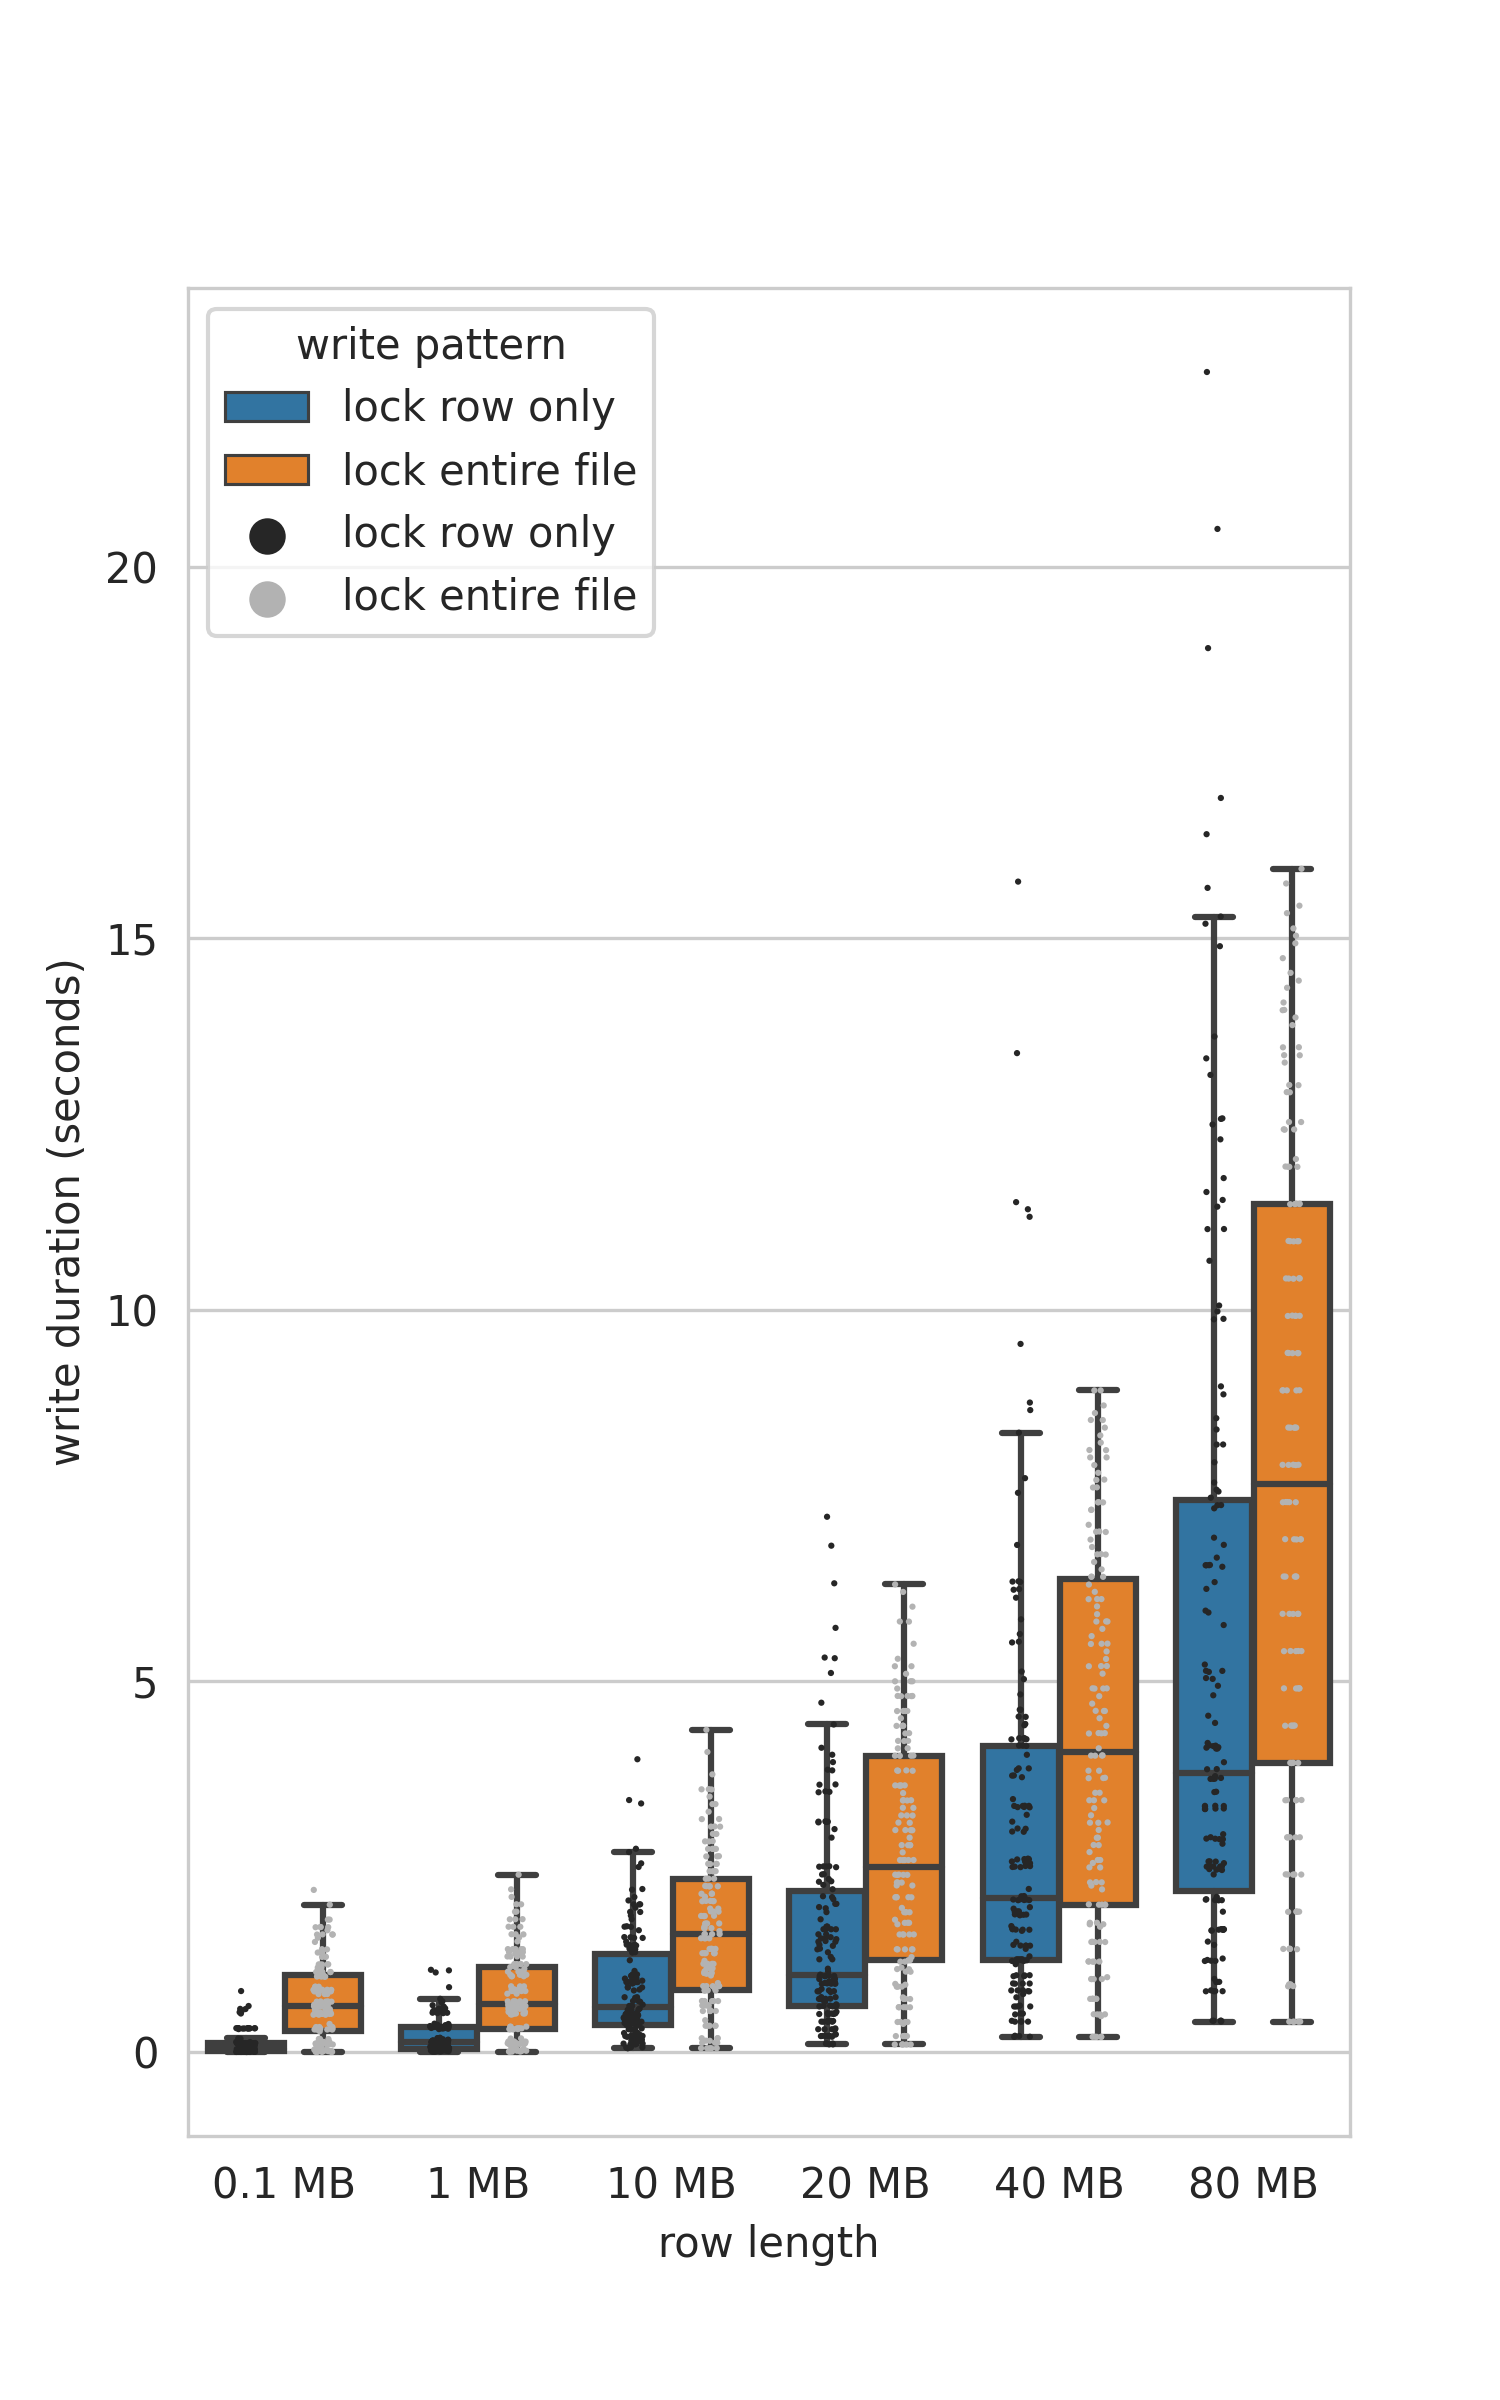
\includegraphics[width=3\textwidth]{../results/plots/single_vs_row_len.png}
	\caption{Time it takes to write a single row given different row sizes. Every dot is a single measurement. On the Y-axis the duration a single write request takes in seconds.}
	\label{fig:single_rowlen}
\end{figure}
%
In \Cref{fig:single_writers} we see that with more simultaneous writers locking only a single row becomes faster. Note how locking the entire file is faster up to and including 4 writers. These results where triple checked.
%
\begin{figure}[htbp]
	\centering
	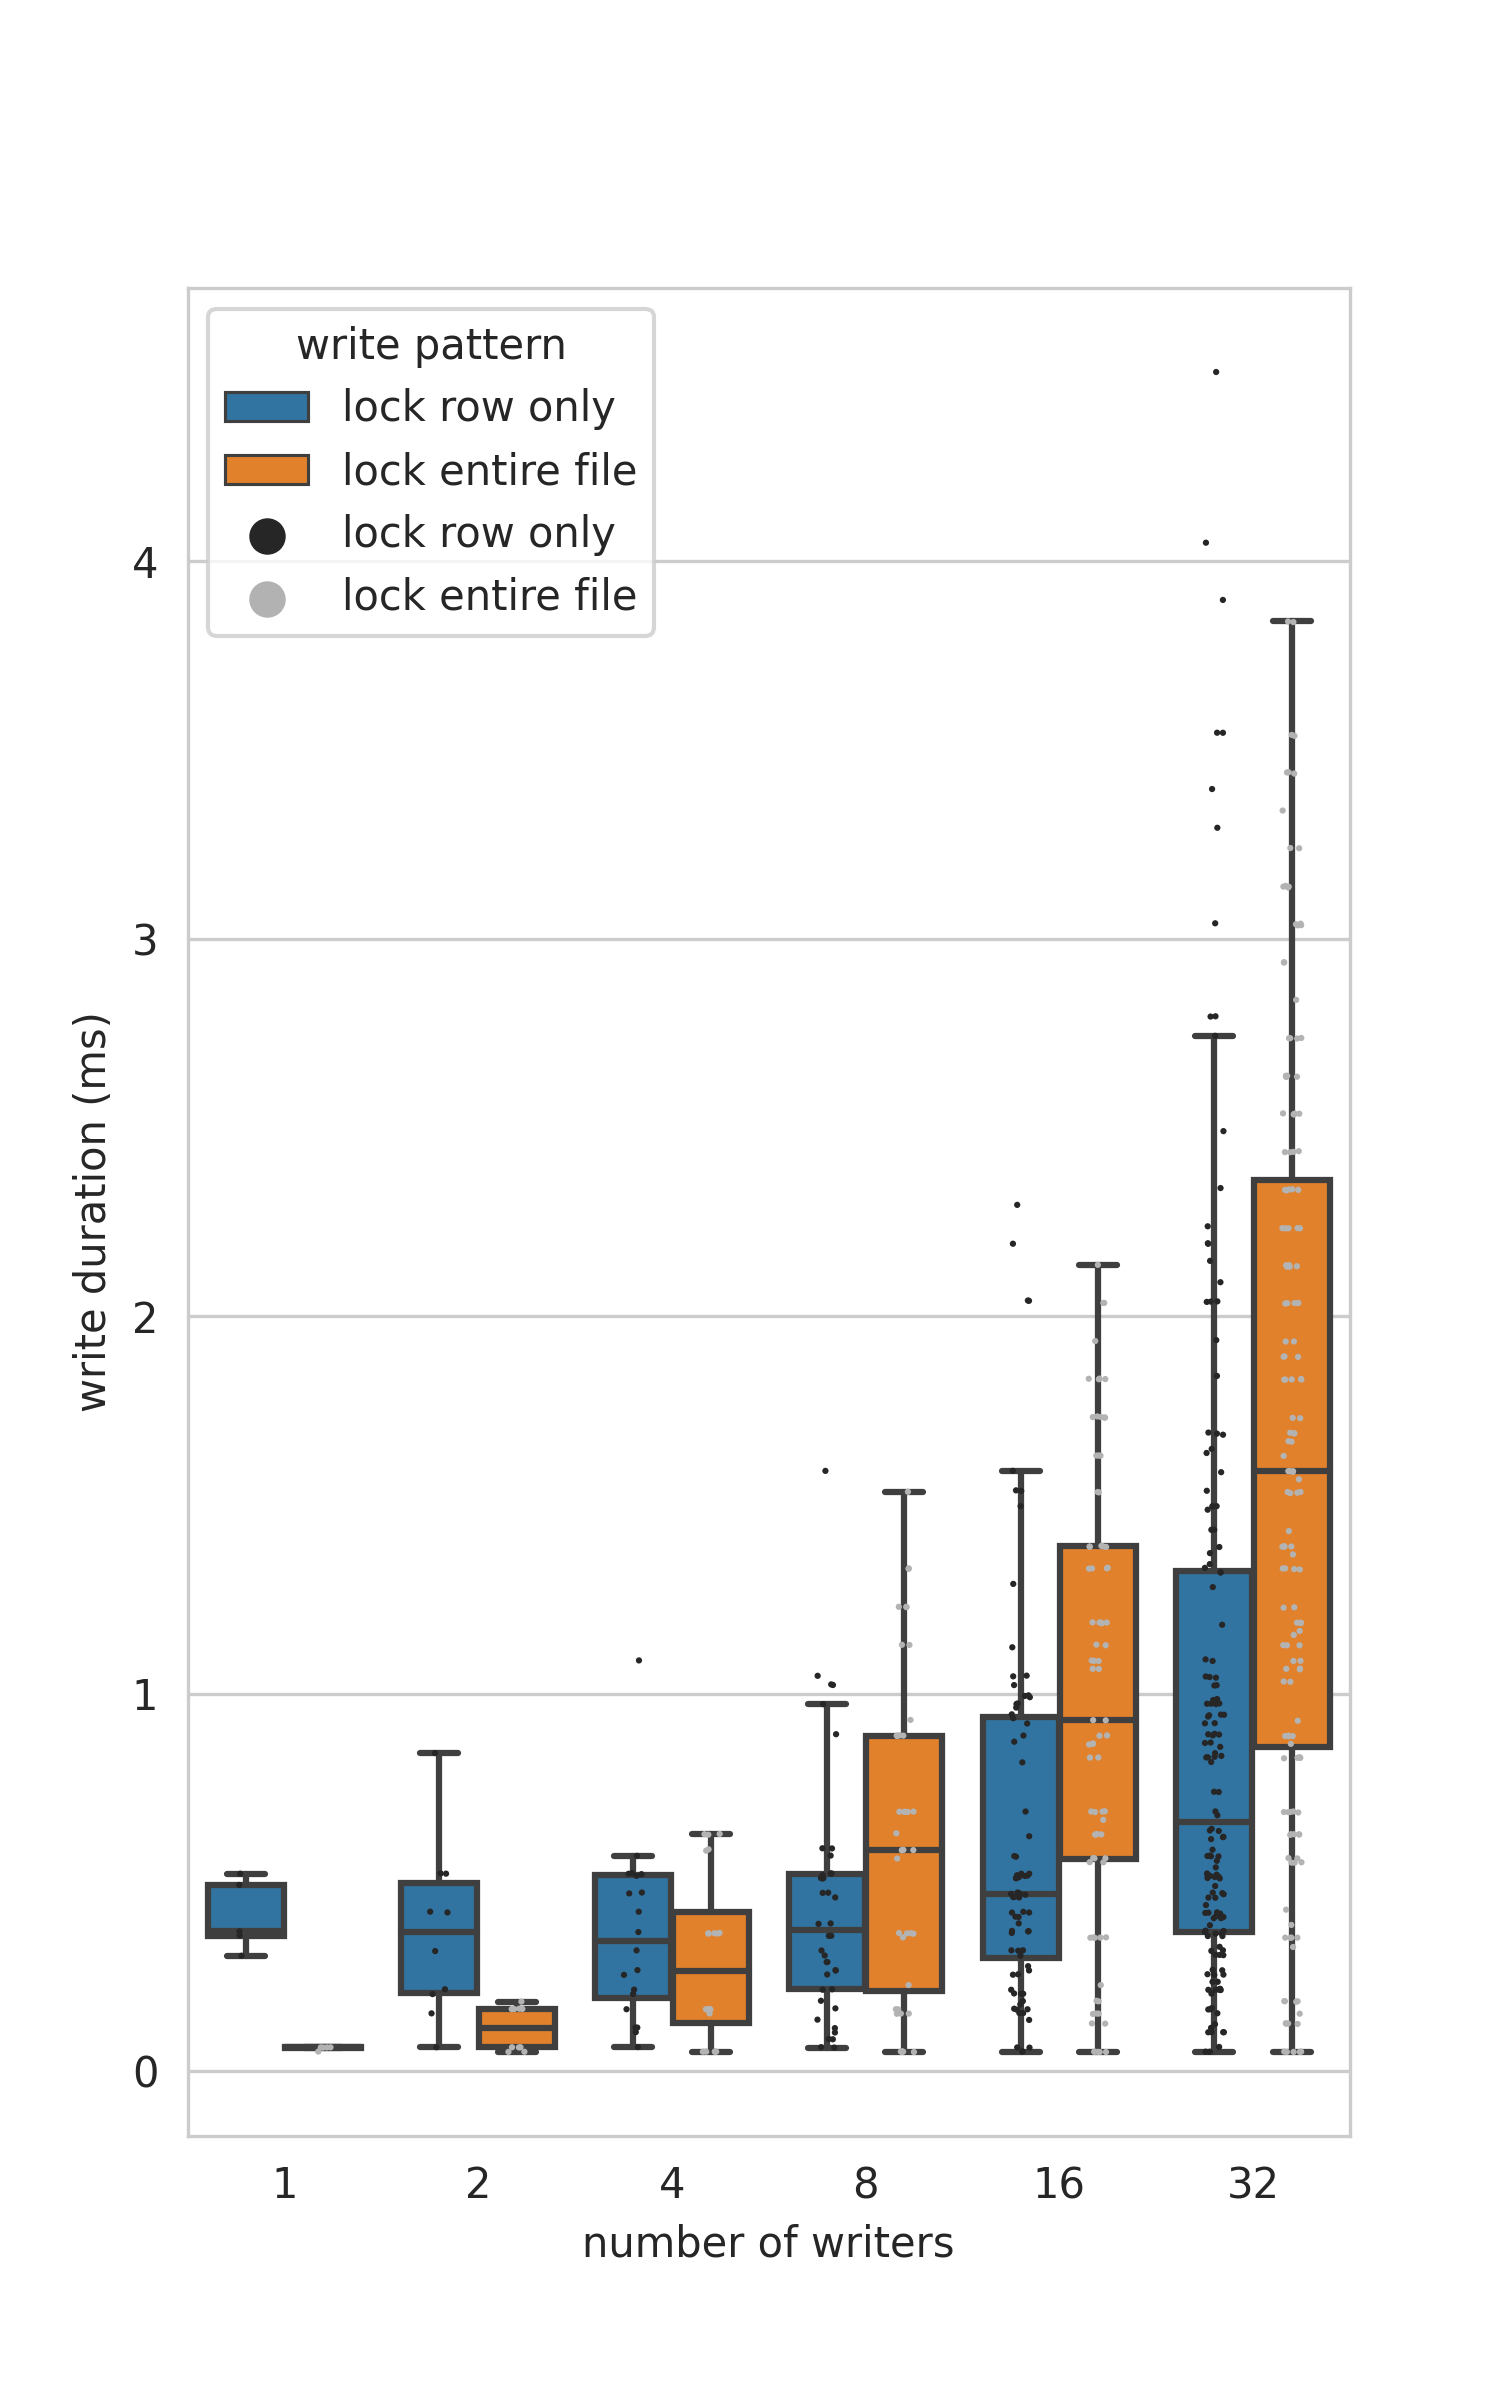
\includegraphics[height=\textheight]{../results/plots/single_vs_writers_both.png}
	\caption{Time it takes to write a single row given different numbers of writers from 1 to 32. On the Y-axis the duration in milliseconds. In blue results for only locking the needed row while in orange we see the times when locking the entire file.}
	\label{fig:single_writers}
\end{figure}

\clearpage
\subsubsection{Writing the entire file}
In \Cref{fig:rowlen} we present every individual duration for writing all 10 rows given various row lengths. Again we compare locking by row vs locking the entire file. The Y-axis logaritmically shows the duration in seconds. The X-axis shows various sizes for the files rows. Note that as expected larger rows result in longer write durations. Furthermore, we see discrete levels in write duration when writing the entire file and not when writing by row.
%
\begin{figure}[htbp]
	\centering
	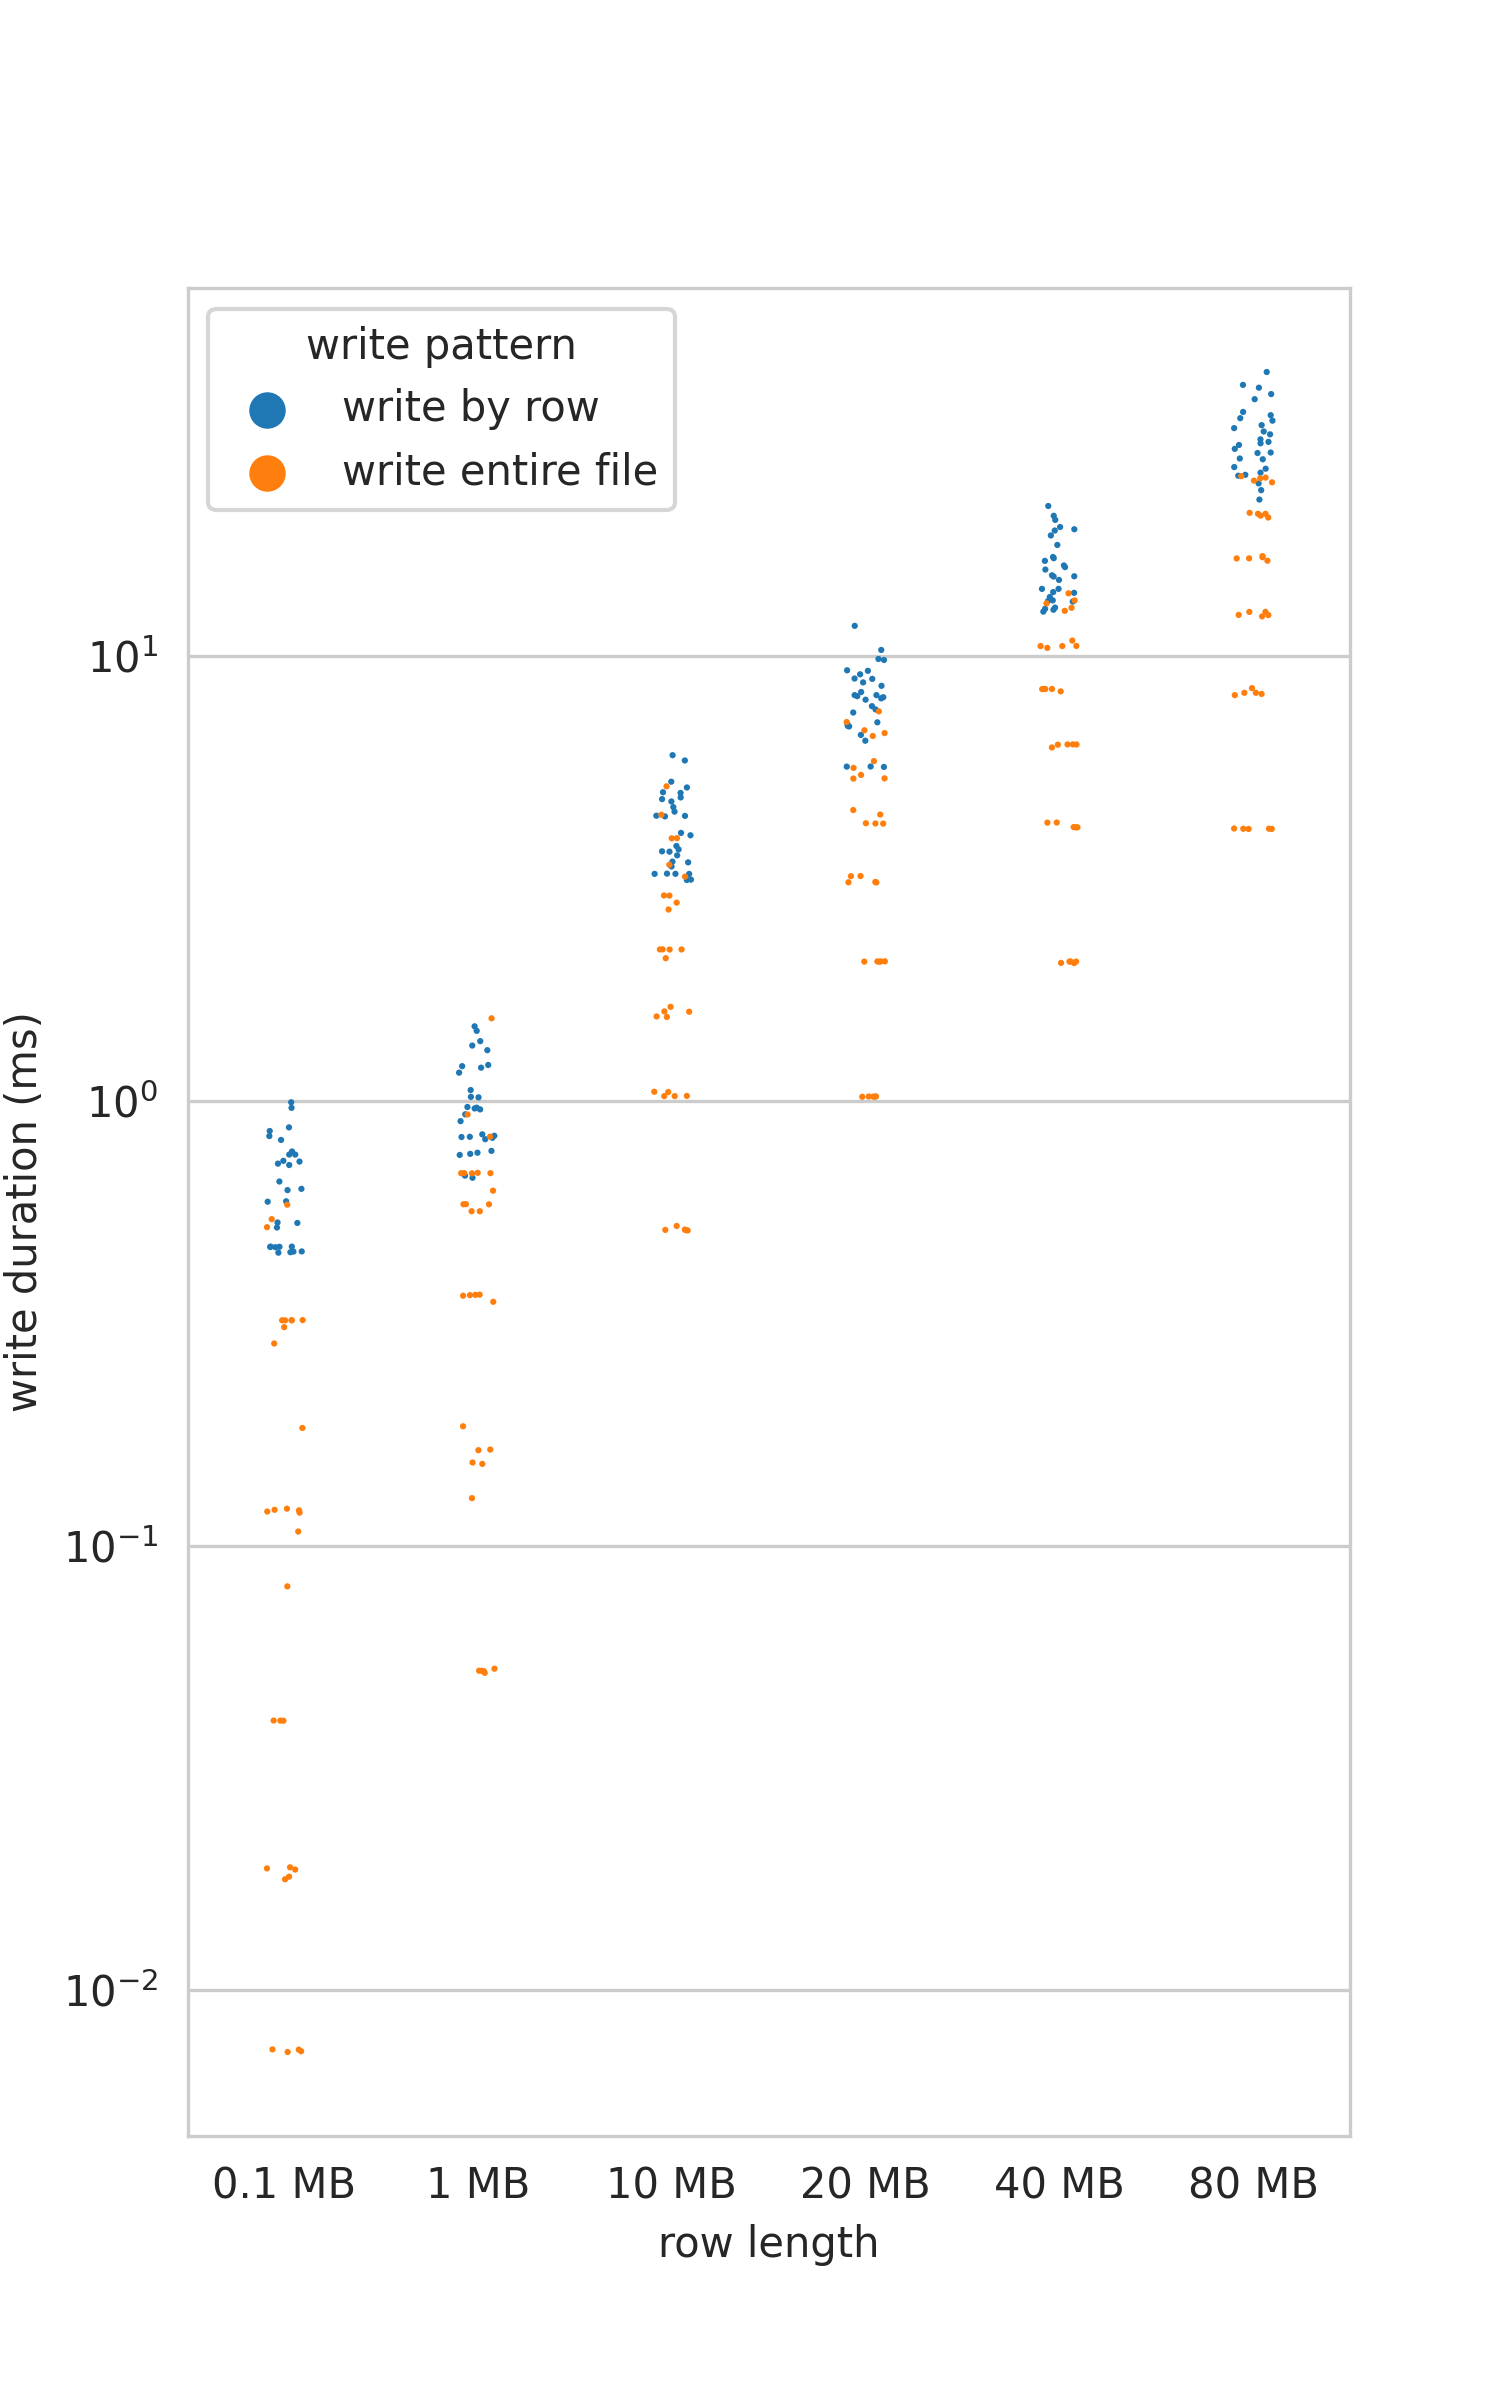
\includegraphics[height=\textheight]{../results/plots/range_vs_row_len.png}
	\caption{The time it takes to write 10 rows for varying row sizes. The blue dots are durations for writing 10 times each time only locking the needed row. In orange the duration when locking the entire file and writing only once.}
	\label{fig:rowlen}
\end{figure}%
%
\Cref{fig:writers} shows the duration it takes to write all the rows, comparing locking by row vs locking the entire file. The Y-axis shows time it takes to write all 10 rows. Note how writing by row takes significantly longer with the gap closing when the number of writers increases.
%
\begin{figure}[htbp]
	\centering
	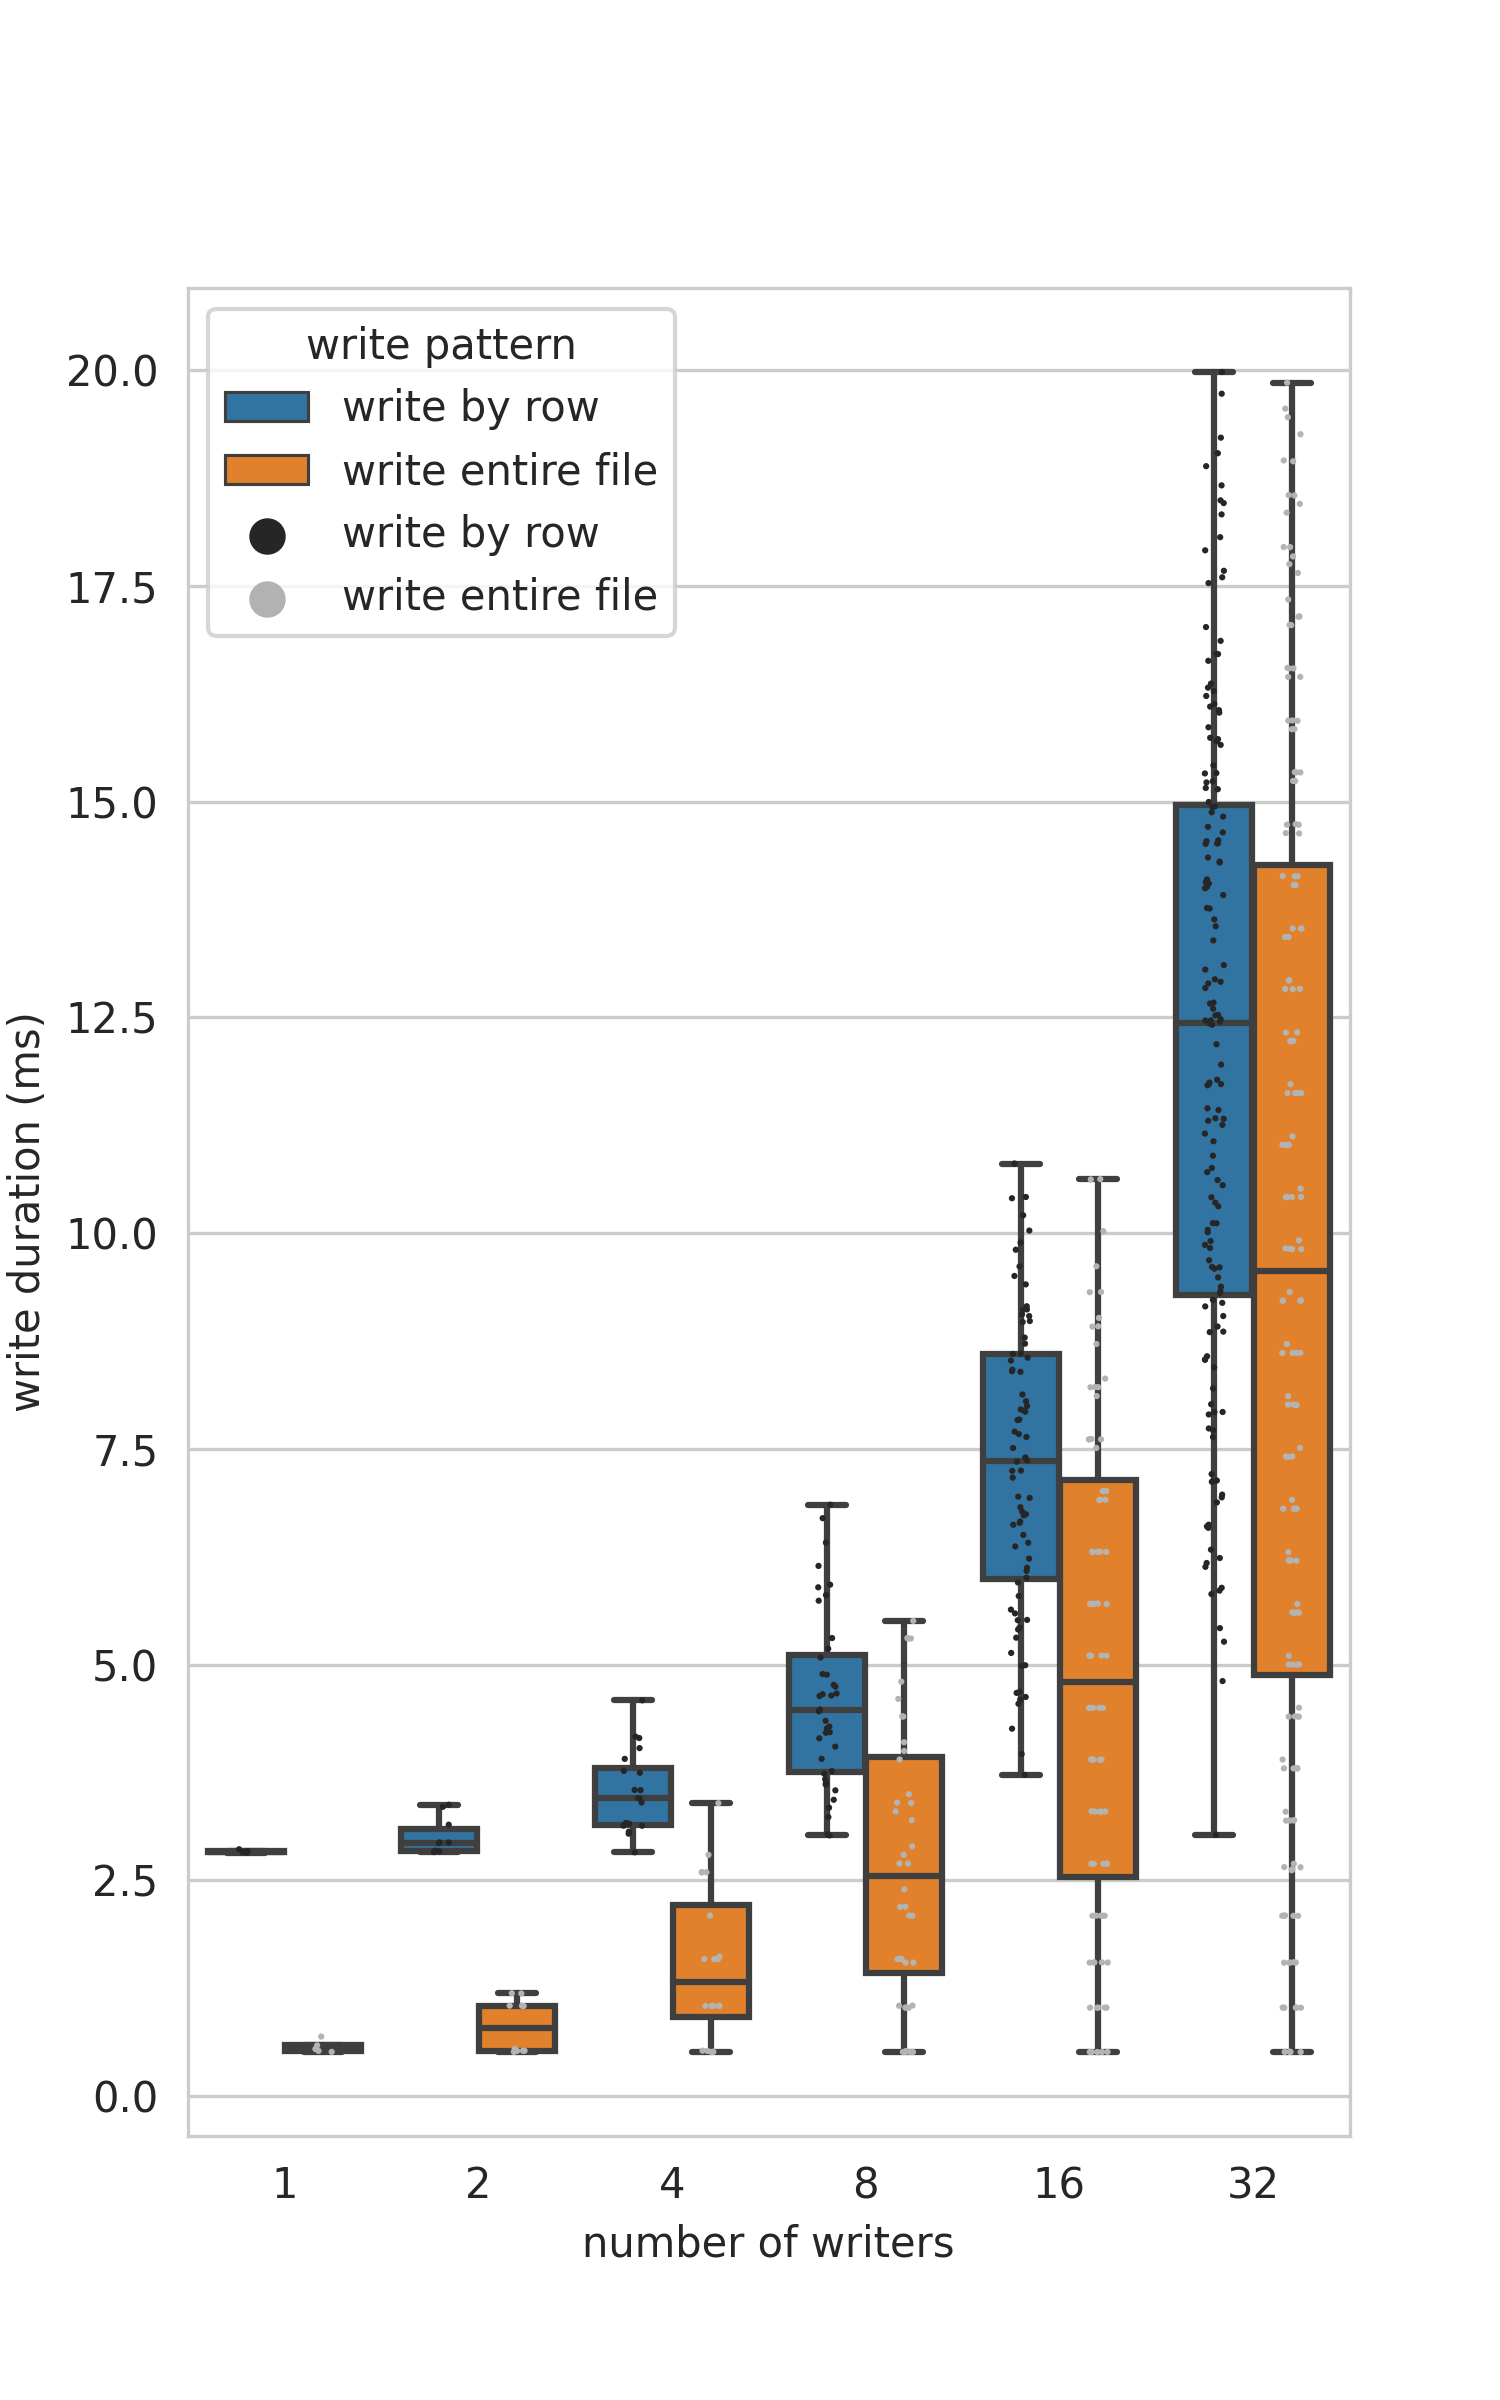
\includegraphics[height=\textheight]{../results/plots/range_vs_writers_both.png}
	\caption{The time it takes to write 10 rows for varying row sizes. The blue dots are durations for writing 10 times each time only locking the needed row. In orange the duration when locking the entire file and writing only once.}
	\label{fig:writers}
\end{figure}

\clearpage

%\subsection{Profiling} \label{sec:profile}
% for now we are not doing this (time limitations)
